\subsection{RQ2: Expected time of availability of adequate resources of new languages}
\label{RQ2}

It is hard to define ``adequate resource'' of a programming language in QA site. However, we can use an indirect approach to measure adequate resource. Two major types of Stack Overflow questions are \emph{repetitive} questions and the \emph{new} questions. By \emph{repetitive} question we mean the same question or same problem but the developers \citep{TausczikWC17} faced this problem in another platform or environment. The decrease in the number of the new question indicates that Stack Overflow already has the answer to most of the questions or problems. From this point of view, we can say that in Stack Overflow we have ``adequate resource'' of that particular language if the number of new questions is within a limit. However,  questions are not the only way developers interact with Stack Overflow.
There are other ways like votes and comments. To reflect the contribution of all the means of interaction into determining the expected time for the availability of the adequate resource, we have followed the approach of Srba et al.\citep{Srba2016}. Using this approach, we have calculated average post (by post we mean both question and answer) quality in Stack Overflow. \textcolor{green}{To measure post quality, we need to consider all types of interactions within a given time frame. This deadline is necessary to ensure equal duration for all posts; Otherwise, old questions will have more opportunities for comments and answers than new questions. In SO, however, a post may receive a vote long after the date it was created; for example, in our dataset, a post received a vote from a user twelve years later. Such a long duration reduces the length of the data set. However, most votes, comments, and answers are available after a certain period. As stated by \citep{Bhat2014} 63.5\% question receives answer within one hour, and only 9.98\% question receives answer after one day.} We quantified post quality by calculating the \emph{score} for each month. To calculate post quality (\emph{score}) from votes of answers, accepted answers and comments, we have considered the votes received within \textcolor{green}{thirteen day} of the creation of post. \textcolor{green}{To fix the \emph{thirteen-day} as period, we calculated the distribution of the accepted answer time, answer time and comment time.\emph{The thirteenth day} is the 85 percentile of answer time, 95 percentile of accepted answer time, 90\% percentile of the comment time. We calculated the post quality increasing the duration but post quality did not change significantly.} \emph{Score} represents the average post quality, and \emph{interaction score} represents the average developers' interaction of that language. To calculate \emph{score}, votes from accepted answers are given double weight compared to those without an accepted answer. This practice exists\citep{Romano2013}  to prioritize the  contribution of accepted answers. The detail calculation of \emph{score} and \emph{interaction score} is presented below.

\noindent
Let, \\
$Q = $ {All questions of a month},\\
$A = $ {All answers of questions in $Q$ where creation date is within 13 days of  $Q$},\\ 
$C = $ {All comments of both $Q$ and $A$ within 13 days of $A$},\\
$S = $ {All accepted answers of $Q$ where creation date is withing 13 days of $Q$},\\
$T(x) = $ Creation time of item $x$.\\
Now,\\


\begin{equation}
\begin{split}
Interaction\ Score = \dfrac{\sum_{Q_i\in Q}Q_i+ \sum_{A_i\in A}A_i+\sum_{C_i\in C}C_i}{\sum_{Q_i\in Q}Q_i}
\end{split}
\end{equation}

\begin{equation}
\begin{split}
and,\ & Score = \dfrac{\sum_{Q_i\in Q}\sum_{\substack{Q_v\in Votes\: of\: Q_i\\T(Q_v) \leq T(Q_i)+13}}Q_v}{\sum_{Q_i\in Q}Q_i}+  \dfrac{\sum_{A_i\in A}\sum_{\substack{A_v\in Votes\: of\: A_i\\T(A_v) \leq T(A_i)+13}}A_v}{\sum_{Q_i\in Q}Q_i}+\dfrac{\sum_{S_i\in S}\sum_{\substack{S_v\in Votes\: of\: S_i\\T(S_v) \leq T(S_i)+13}}S_v}{\sum_{Q_i\in Q}Q_i} 
\end{split}
\end{equation}


%Interaction Score = $\dfrac{\sum_{Q_i\in Q}Q_i+ \sum_{A_i\in A}A_i+\sum_{C_i\in C}C_i}{\sum_{Q_i\in Q}Q_i}$\\
% and, Score = $\dfrac{\sum_{Q_i\in Q}\sum_{\substack{Q_v\in Votes\: of\: Q_i\\T(Q_v) \leq T(Q_i)+24}}Q_v}{\sum_{Q_i\in Q}Q_i}+$\\  
% $\dfrac{\sum_{A_i\in A}\sum_{\substack{A_v\in Votes\: of\: A_i\\T(A_v) \leq T(A_i)+24}}A_v}{\sum_{Q_i\in Q}Q_i}+\dfrac{\sum_{S_i\in S}\sum_{\substack{S_v\in Votes\: of\: S_i\\T(S_v) \leq T(S_i)+24}}S_v}{\sum_{Q_i\in Q}Q_i}$\\


\begin{figure}[htbp]
\begin{subfigure}{0.6\textwidth}
\centering
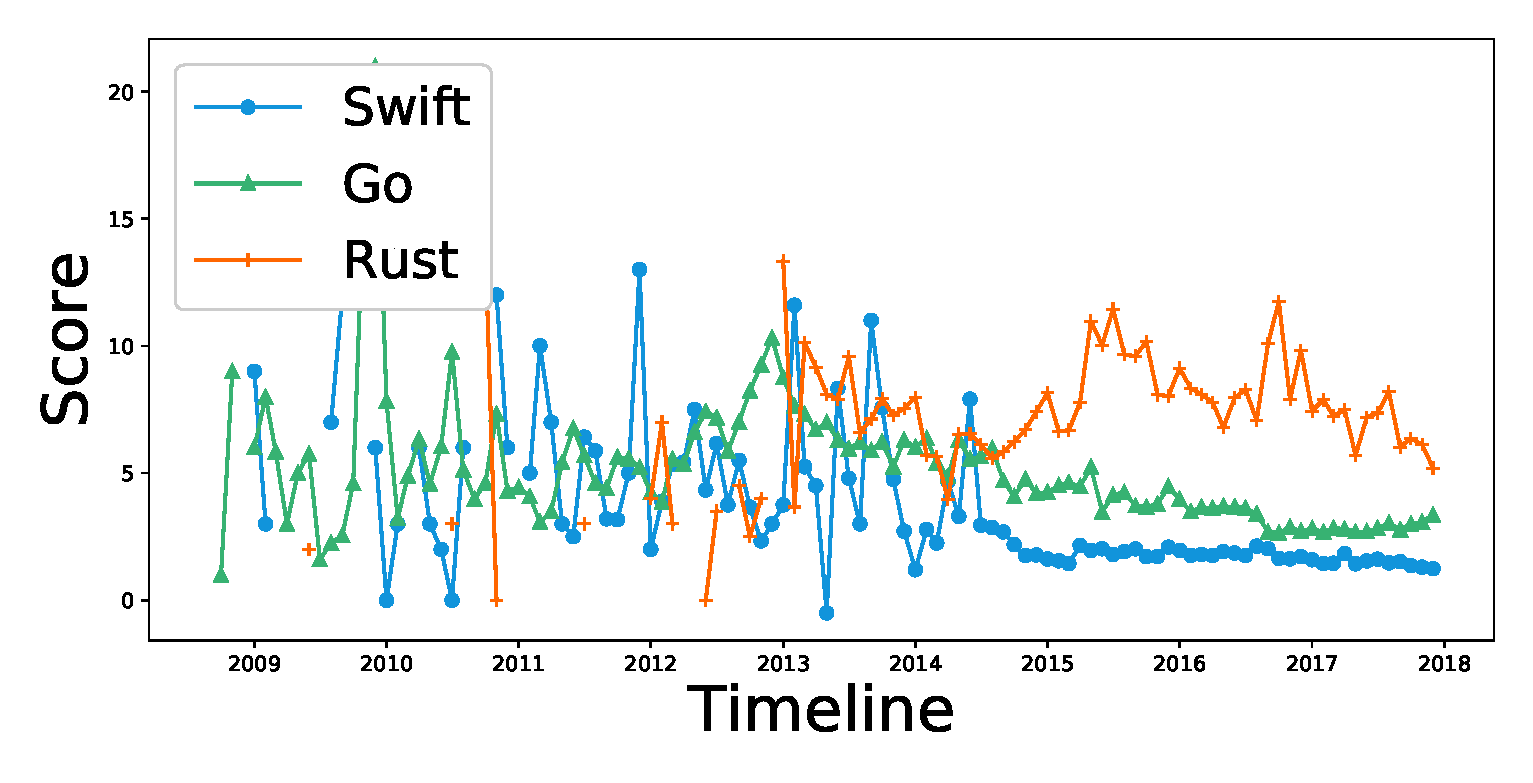
\includegraphics[scale=0.2]{figures/content_quality.eps}
\caption{Post quality of new languages in Stack Overflow}
\label{fig:Content quality}
\end{subfigure}
\begin{subfigure}{0.6\textwidth}
\centering
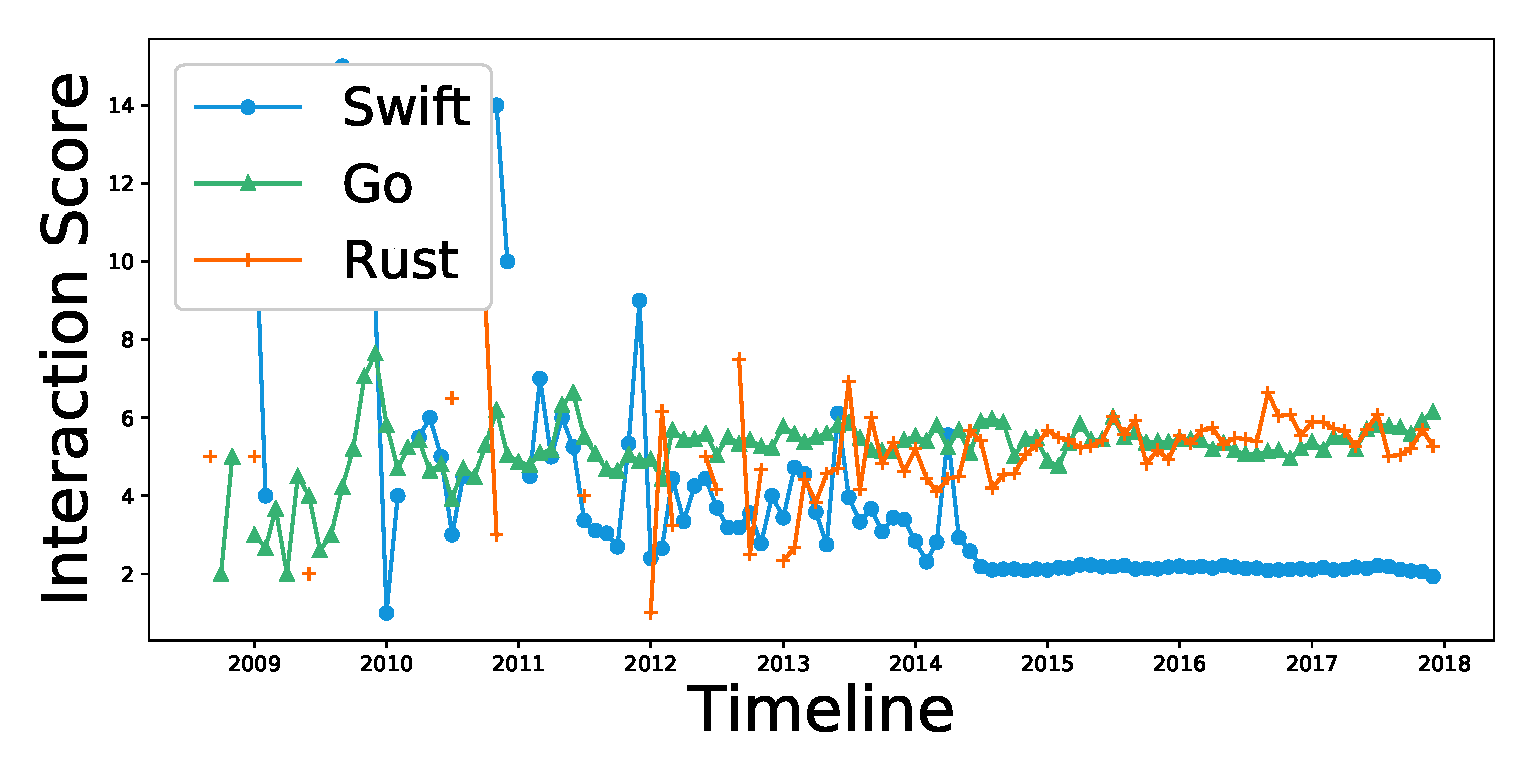
\includegraphics[scale=0.2]{figures/interaction.eps}
\caption{Interaction of developers of new languages with Stack Overflow}
\label{fig:Interaction}
\end{subfigure}
\caption{Post quality of new languages and developers' interaction with new languages vs. time }
\end{figure}

From Figure~\ref{fig:Content quality} it is quite clear that after the release of language, post quality is unstable and the values are very high. The reason behind instability is that the language lacks resources and every new release triggers a set of new questions. The questions of the starting years are less repetitive than the later years\citep{Srba2016}, and it is the reason behind the high value of \emph{score}. Gradually \emph{score} stabilizes into a certain point. In a stable language, users' interaction with Stack Overflow should be minimum and within a range. From Figure~\ref{fig:Interaction}, it is evident that after the first release, \emph{interaction score} also stabilizes to a point which supports our conjecture.

%Continuous up gradation of a feature, documentation  leads a language to its stable point.
To effectively measure the difference of score between consecutive months \emph{first difference} metric \citep{Rasheed2011} has been applied on the score of each language. First difference of score is the difference of score of the consecutive month. \textcolor{green}{The \emph{first difference} technique removes any unobserved variable from data. Moreover, as the data points are taken at a constant interval, the value of the \emph{first difference} works like a differential value.} The first difference is plotted against the release time in Figure~\ref{First difference and release}. In the beginning, the first difference of score was following the release. However, gradually it decreases the level of response which means the language is stabilizing. We can detect a stable point for a language from this point of view. By the stable point, we mean the starting date of the period after the first release of a language when the language is so stable that a single release cannot change or disrupt the development process.

If the first difference of score of a language is within a range, then it has two meanings. First, the language is stable. It does not initiate any significant change in the development lifecycle. Secondly, since most of the Stack Overflow posts are repeated, the contribution of this kind of questions will be omitted in the first difference process. Now, we have the effect of the change of frequency of new questions in the first difference of score. Therefore, the first difference of score within a range means developers are facing fewer problems which are not already answered in Stack Overflow. Hence, we can say we have adequate resources in Stack Overflow on new languages.

\begin{figure}[htbp]
\begin{subfigure}{0.6\textwidth}
\centering
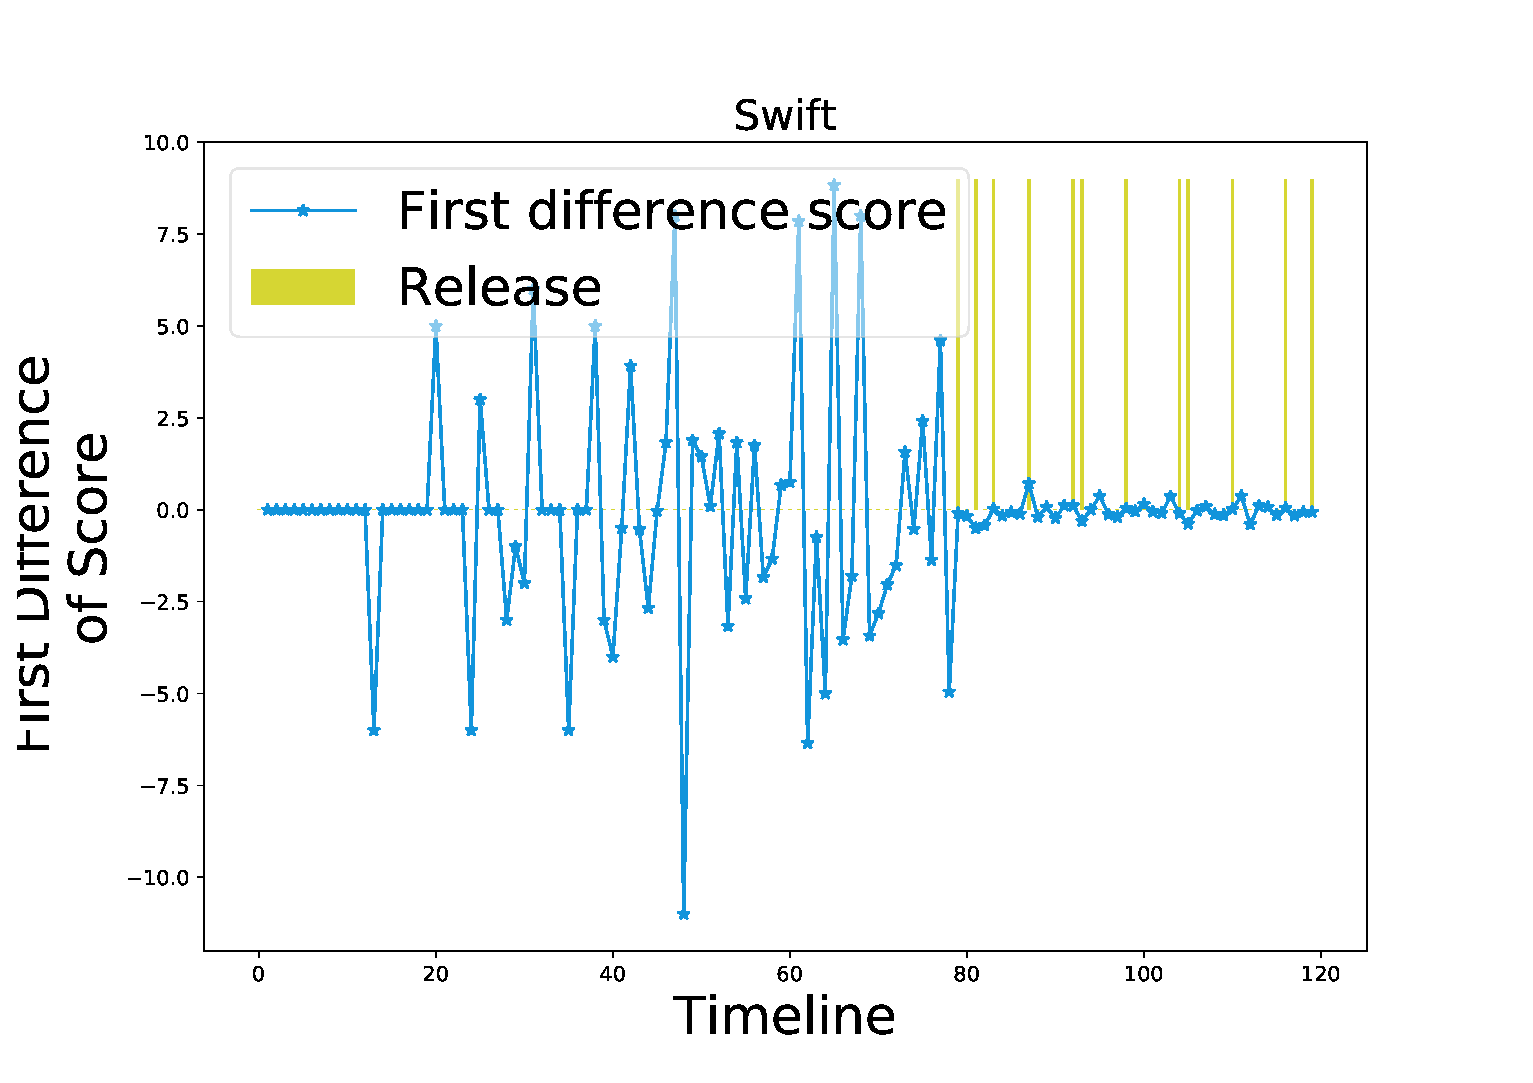
\includegraphics[scale=0.25]{figures/Swift_First_difference_release.eps}
\caption{Swift}
\label{fig:Go_FDR}
\end{subfigure}
\begin{subfigure}{0.6\textwidth}
\centering
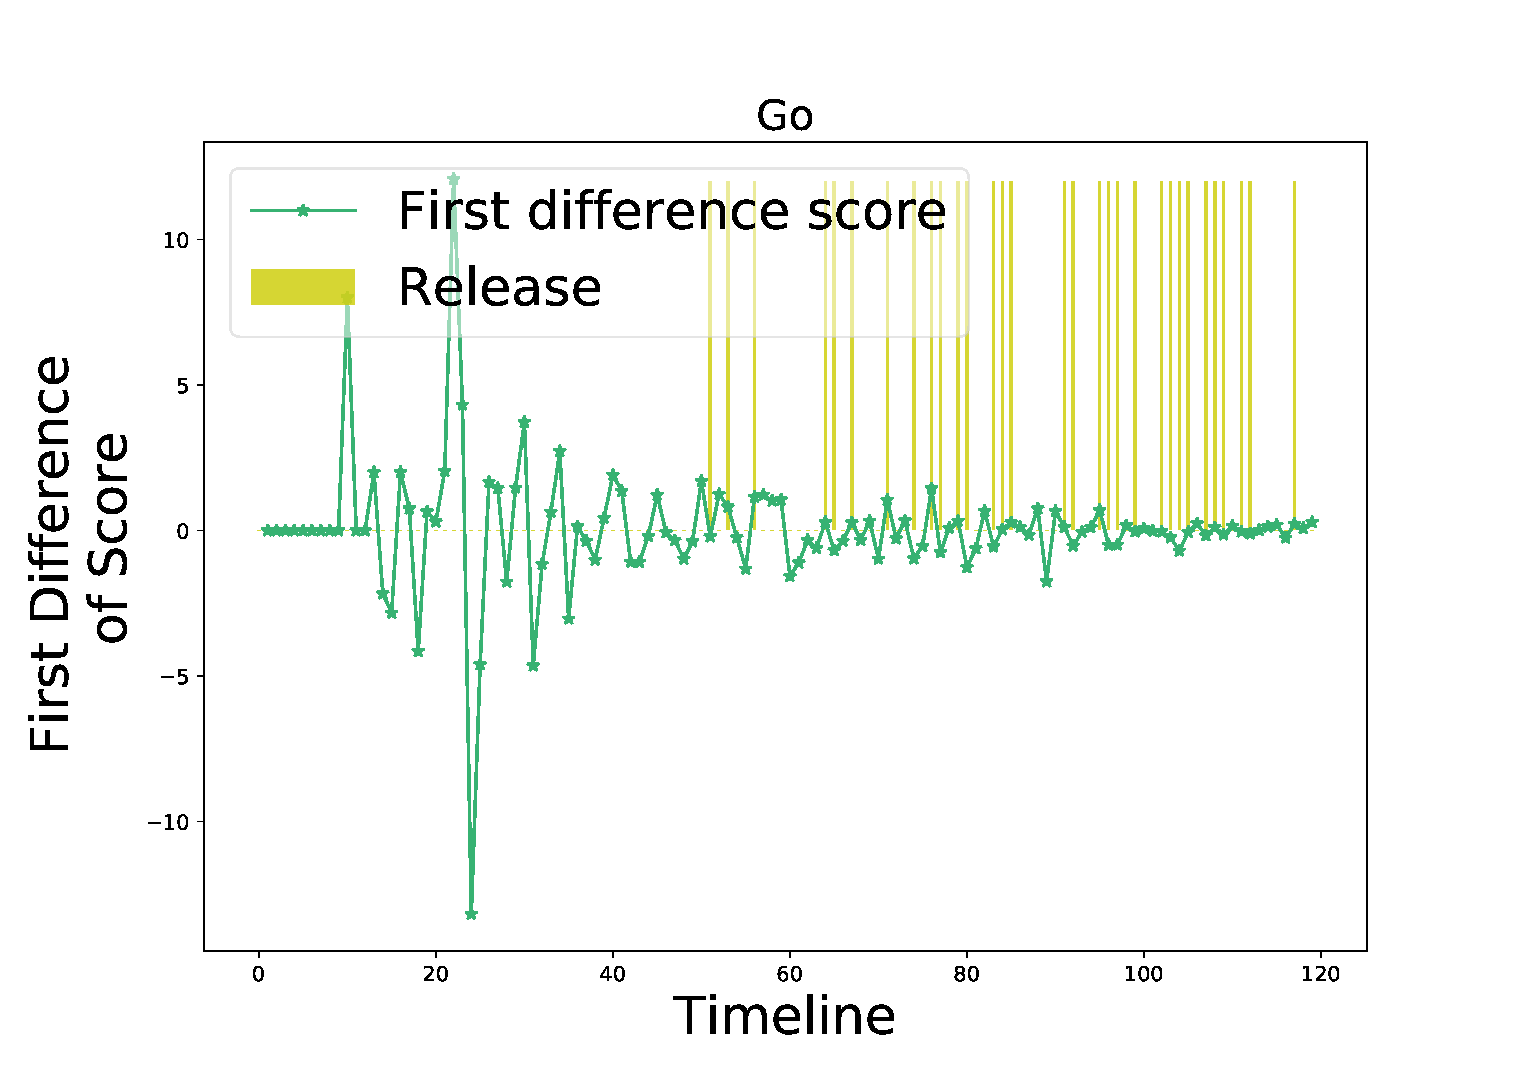
\includegraphics[scale=0.25]{figures/Go_First_difference_release.eps}
\caption{Go}
\label{fig:Swift_FDR}
\end{subfigure}
\begin{subfigure}{0.6\textwidth}
\centering
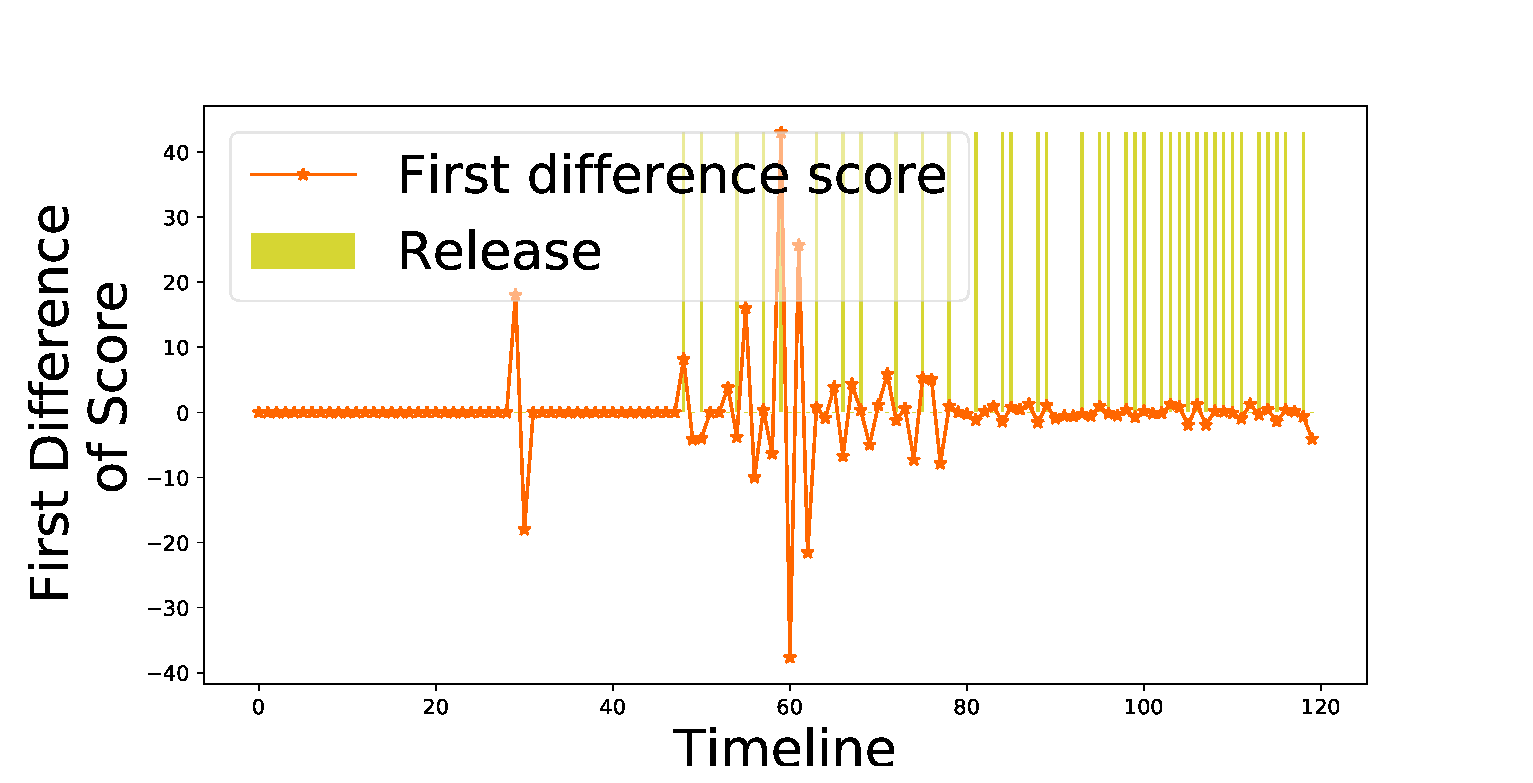
\includegraphics[scale=0.25]{figures/Rust_First_difference_release.eps}
\caption{Rust}
\label{fig:Rust_FDR}
\end{subfigure}
\caption{First difference of the post quality of new languages and release of a new version of new languages.}
\label{First difference and release}
\end{figure}

We defined the stable point as the time point after which value of the first difference is always between -1 and 1. Stable point for each language is presented in Table~\ref{table:Stable point}

\begin{table}[htbp]
\centering
\caption{Stable point of the new languages}
\begin{tabular}{|l|l|l|}
\hline
Language & Release Date & Stable Point Date  \\ \hline
Go & March 1, 2012 & July 1, 2015\\ \hline
Swift & September 9, 2014 & November 1, 2016\\ \hline
Rust & January 1, 2012 & Not reached \\ \hline
\end{tabular}
\label{table:Stable point}
\end{table}

In Stack Overflow the number of Rust developer is too low compared to the other two languages. It is quite common in Stack Overflow that a particular portion of developers leaves or become inactive in  Stack overflow after some time. The post quality of Rust will change quickly after such departure. However, such departure cannot change Go or Swift post quality so frequently as departing developers represent a small percentages of the whole community of these languages in Stack Overflow. That is why our study has found that Rust language has not reached a stable point in Stack Overflow.

\boxtext{\textbf{Finding 2:} In Stack Overflow, we can expect adequate resources of Swift after two years of release while this period is three years for Go. We have found the evidence of having an inadequate resource of Rust language in Stack Overflow.}

\boxtext{\textbf{Finding 3:} The size of an active community can influence the growth of a new language.}

% The significance of stable point is, after the stable point the growth of a language is not affected by a new release. That means quality answers and questions about all the core features are already available in Stack Overflow. We may say a developer will find the answers of all the common questions in Stack Overflow after stable point.ambiguous.